\documentclass[letterpaper,11pt,twoside]{article}
\usepackage[utf8]{inputenc}
\usepackage{amsmath,amsfonts,amssymb,amsthm,latexsym}
\usepackage[spanish,es-noshorthands]{babel}
\usepackage[T1]{fontenc}
\usepackage{lmodern}
\usepackage{graphicx,hyperref}
\usepackage{tikz,pgf}
\usepackage{multicol}
\usepackage{fancyhdr}
\usepackage[height=9.5in,width=7in]{geometry}
\usepackage{fancyhdr}
\pagestyle{fancy}
\fancyhead[LE]{matematicas.german@gmail.com}
\fancyhead[RE]{}
\fancyhead[RO]{\url{https://www.autistici.org/mathgerman}}
\fancyhead[LO]{}

\author{Germ\'an Avenda\~no Ram\'irez~\thanks{Lic. Mat. U.D., M.Sc. U.N.}}
\title{\begin{minipage}{.2\textwidth}

\includegraphics[height=1.75cm]{Images/logo-colegio.png}\end{minipage}
\begin{minipage}{.55\textwidth}
\begin{center}
Taller 03, Función afín\\
Álgebra $9^{\circ}$
\end{center}
\end{minipage}\hfill
\begin{minipage}{.2\textwidth}

\includegraphics[height=1.75cm]{Images/logo-sed.png} 
\end{minipage}}
\date{}
\thispagestyle{plain}
\begin{document}
\maketitle
Nombre: \hrulefill Curso: \underline{\hspace*{44pt}} Fecha: \underline{\hspace*{2.5cm}}
\begin{multicols}{2}
 Ya sabemos que la función afín es de la forma
 \[y=mx+b\]
 donde $m$ es la pendiente y $b$ representa el punto en el que es interceptado el eje $y$. Si $b$ es cero, la función además es \emph{lineal}.
 \section*{Aplicaciones de la función afín}
 \subsection*{Ejemplo}
 El costo en pesos por hacer funcionar una bombilla de 60 watios está dado por la función $c(h)=9.0612h$ donde $h$ representa el número de horas que dura encendida la bombilla. Resuelva:
 \begin{itemize}
 \item[a.] ¿Cuál es el costo que se debe pagar por hacer funcionar una bombilla de 60 watios durante treinta días (un mes) tres horas diarias?
 \item[b.] Grafique la función $c(h)=9.0612h$
 \item[c.] Suponga que un bombilla de 60 watios funciona en un cuarto cerrado durante una semana hasta que una persona la descubre y la apaga. Utilice el gráfico de la parte b) para aproximar el costo de haber dejado encendida la bombilla durante una semana. Luego use la función para encontrar el costo exacto.
  \end{itemize}
 \subsubsection*{Solución}
 \begin{itemize}
\item[a.]  $c(90)=9.0612(90)=815.508$ Es decir el costo es aproximadamente ochocientos quince pesos con 51 centavos.
\item[b.] Ya que $c(0)=9,0612(0)=0$ y $c(100)=9.0612(100)=906.12$, se pueden usar estos dos puntos A(0,0) y B(100,906.12) para hacer la gráfica de la función ya que sabemos que es una recta con pendiente $m=9.0612$ y el punto de corte $b$ es 0.
\begin{center}
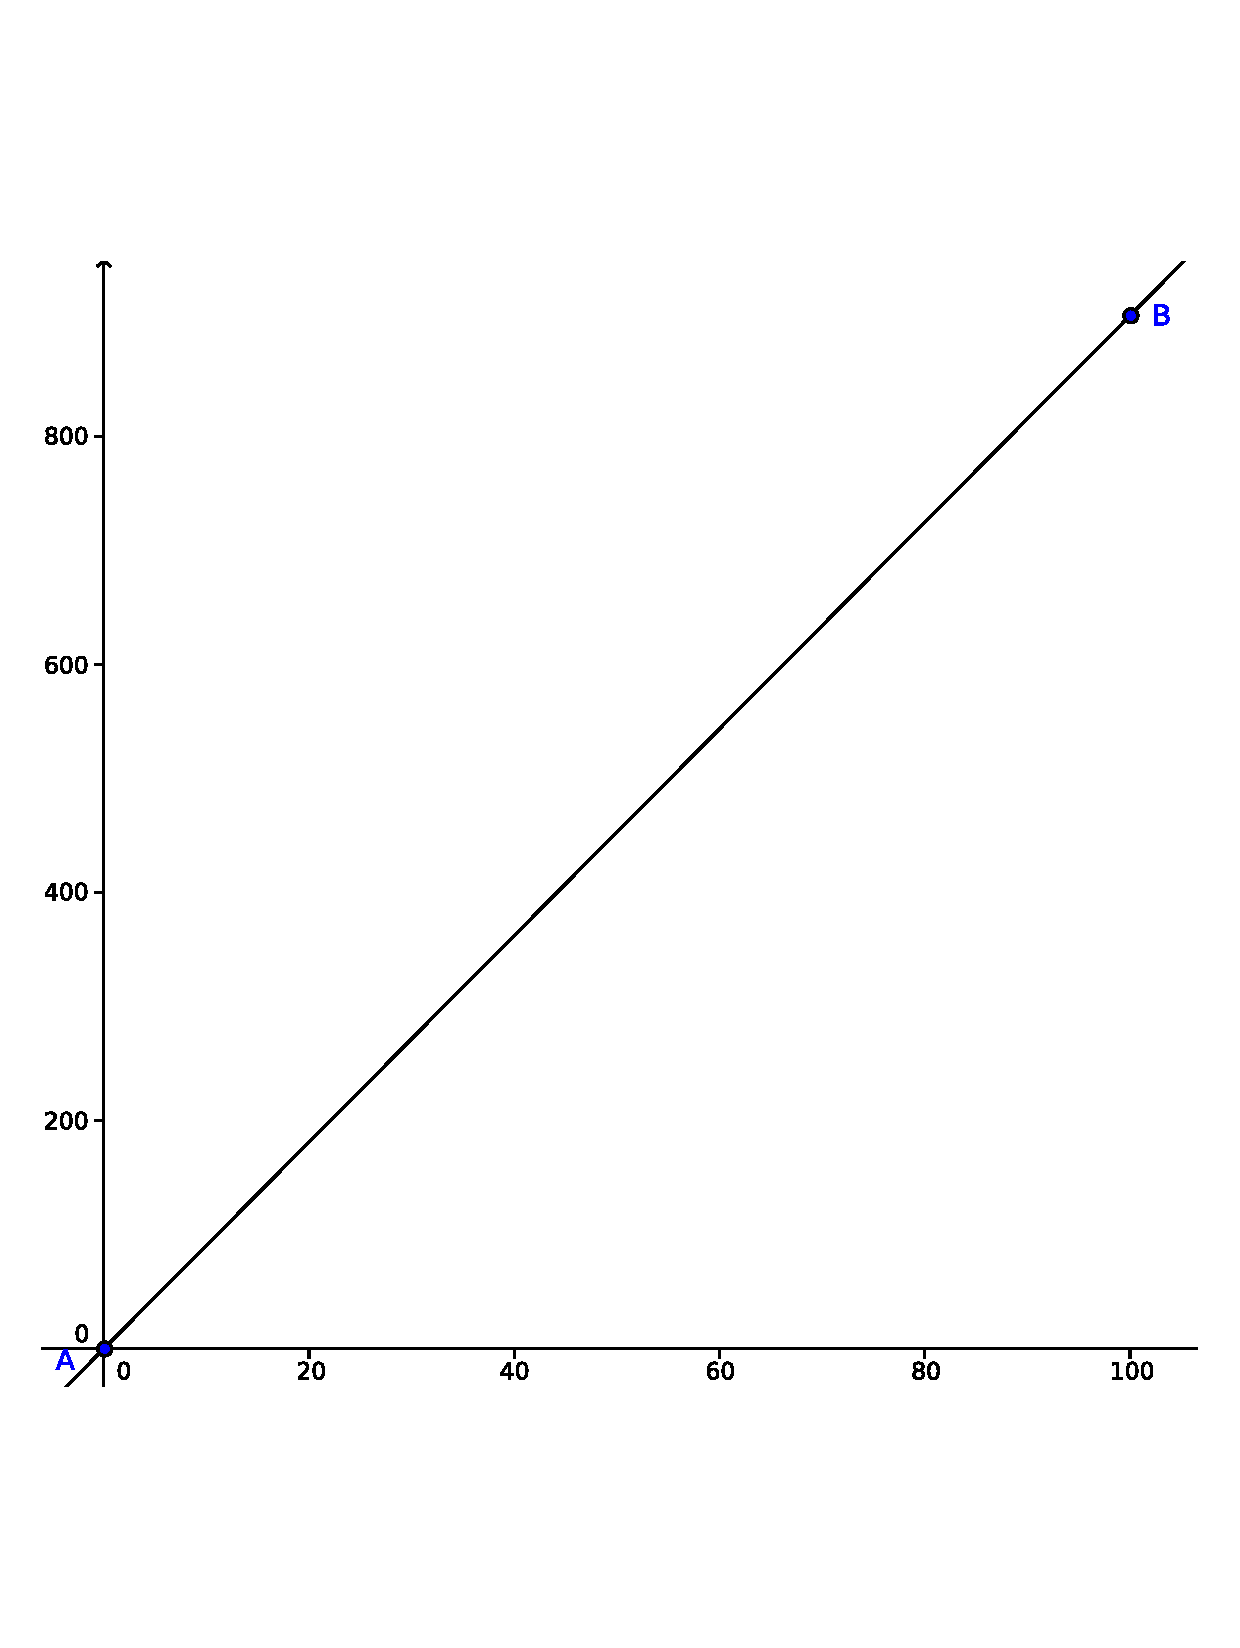
\includegraphics[trim=0cm 2.5cm 0cm 3.5cm, scale=.45]{Images/bombilla-graph.pdf} 
\end{center}
\item[c.] Si la bombilla dura encendida 24 horas al día durante una semana, esta dura $24(7)=168$ horas encendida. Con base en la gráfica se puede calcular aproximadamente cual es el costo; sin embargo la podemos calcular exactamente, usando su ecuación:
\[c(168)=9.0612(168)=1522.2816\]
es decir el costo de haber debajo el bombillo encendido durante una semana es \$1522.28 (mil quinientos veintidos pesos con veintiocho centavos)
 \end{itemize}
 \subsection*{Actividad}
 \subsubsection*{Quiz Conceptual}
 Para los siguientes items, conteste Verdadero (V) o Falso (F)
 \begin{enumerate}
 \item Cualquier función de la forma $f(x)=ax^{n}+b$, donde $a$, $b$ y $n$ son números reales es una función afín.
 \item Geométrica el valor de una función es la distancia directa del eje $y$
 \item La gráfica de una recta horizontal representa una función
 \item La función afín $f(x)=1$ es denominada la función identidad.
 \item Las gráficas de las funciones $f(x)=mx+b$ y $g(x)=-mx+b$ son perpendiculares
 \item Toda línea recta representa una función
 \item La ecuación $f(x)=ax+b$ también puede ser escrita como $y=ax+b$
 \item La gráfica de la función afín $f(x)=-4x+5$, es una línea recta con pendiente $-4$
 \end{enumerate}
 \subsubsection*{Problemas}
 Para los problemas \ref{ex01}--\ref{ex02}, grafique cada función afín
 \begin{enumerate}
 \item $f(x)=3x+3$ \label{ex01}
 \item $f(x)=-2x+6$
 \item $f(x)=2x-6$
 \item $f(x)=-x-5$
 \item $f(x)=-4x$
 \item $f(x)=-1$
 \item $f(x)=\frac{2}{3}x+4$
 \item $f(x)=-\frac{1}{2}x-1$
 \end{enumerate}
 \end{multicols}
\end{document}
